\lab{Algorithm}{Kruskal's and Prim's Algorithm}{Kruskal's and Prim's Algorithm}
\label{Ch:Kruskal}

\objective{Find a minimum spanning tree for a connected weighted graph using Kruskal's Algorithm and Prim's Algorithm.}

\section*{Weight Graphs and Spanning trees}

Remember that a graph is composed of two sets: a set of nodes and a set of edges that connect these nodes. 

\begin{figure}[H]
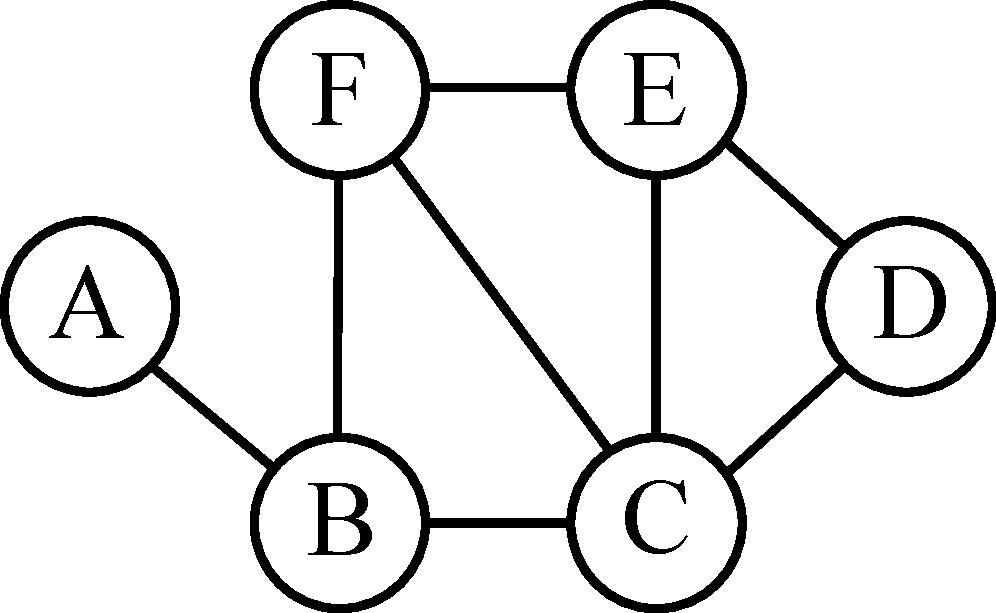
\includegraphics[width = .4\textwidth]{graph1.pdf}
\caption{An example of a graph}
\label{mst:graph1}
\end{figure}

A graph is directed if connections are uni-directional, and undirected if they are bi-directional.
Figure \ref{mst:graph1} shows an undirected graph.
A weighted graph is a graph where each edge has a value associated with it.
Usually these values represent some sort of cost or distance.
A connected graph is a graph where there is a path, or a set of edges, that connect every two nodes together.
We can write a matrix that describes this type of graph.
We let each row of our matrix represent a starting point and each column represent a destination.
If a path from one node to another exists, we put the weight of the path.
If there is no path, we put a 0.
For the above graph we generate the following matrix:

\[
A = \begin{pmatrix}
0 & 1 & 0 & 0 & 0 & 0\\
1 & 0 & 1 & 0 & 0 & 1\\
0 & 1 & 0 & 1 & 1 & 1\\
0 & 0 & 1 & 0 & 1 & 0\\
0 & 0 & 1 & 1 & 0 & 1\\
0 & 1 & 1 & 0 & 1 & 0\\
\end{pmatrix}
\]

This matrix is called an adjacency matrix.
Note that this matrix is symmetric, since the graph is undirected. 

Another way to store the graph is as a list of the edges and their weights that are connected (for an unweighted graph you can just store the edges).
It would look like this:

\begin{align*}
[('A', 'B'),
 ('B', 'C'),
 ('B', 'E'),
 ('B', 'F'),
 ('C', 'D'),\\
 ('C', 'E'),
 ('C', 'F'),
 ('D', 'E'),
 ('E', 'F')]
\end{align*}

A third entry would store the weight.

For this lab, we will be focusing on undirected weighted graphs. 

A spanning tree of a connected undirected graph $G$ is an undirected graph that contains all the nodes of $G$, a subset of the edges, and no cycles.
A cycle, for undirected graphs, is a path where you start and end on the same node without crossing any edge more than once.
Figure \ref{mst:graph3} shows a cycle in an undirected graph.

\begin{figure}[H]
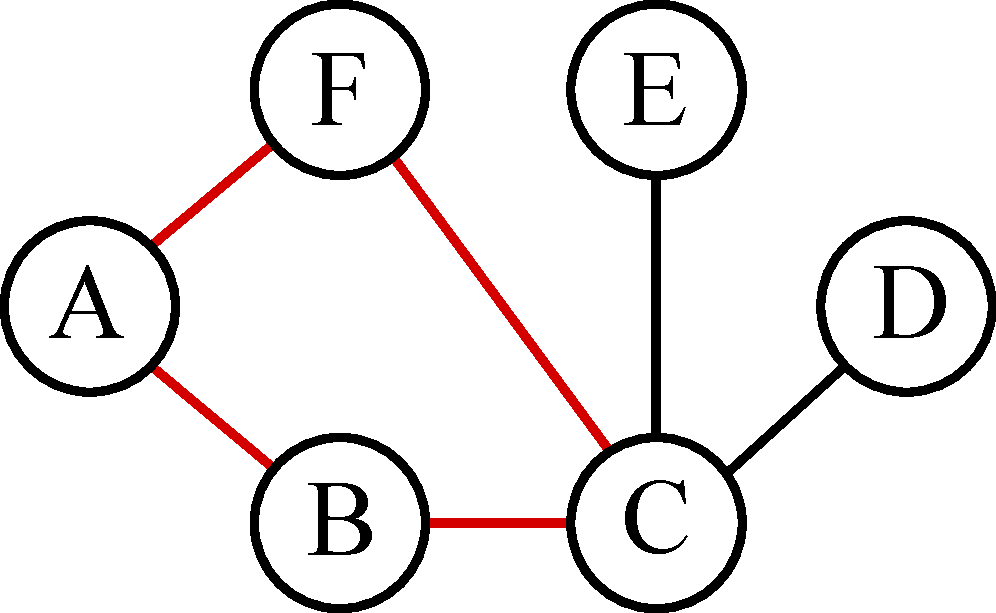
\includegraphics[width = .4\textwidth]{graph3.pdf}
\caption{A cycle in an undirected graph}
\label{mst:graph3}
\end{figure}

The minimum spanning tree (MST) of a weighted, undirected graph is a spanning tree where the sum of the weights of the subset of edges is less than or equal to the sum of the weights of every other spanning tree.
Both Kruskal's and Prim's Algorithms are methods that find the minimum spanning tree of a weighted directed graph.
Figure \ref{mst:graph2} shows a minimum spanning tree of the graph shown in \ref{mst:graph1}.

\begin{figure}[H]
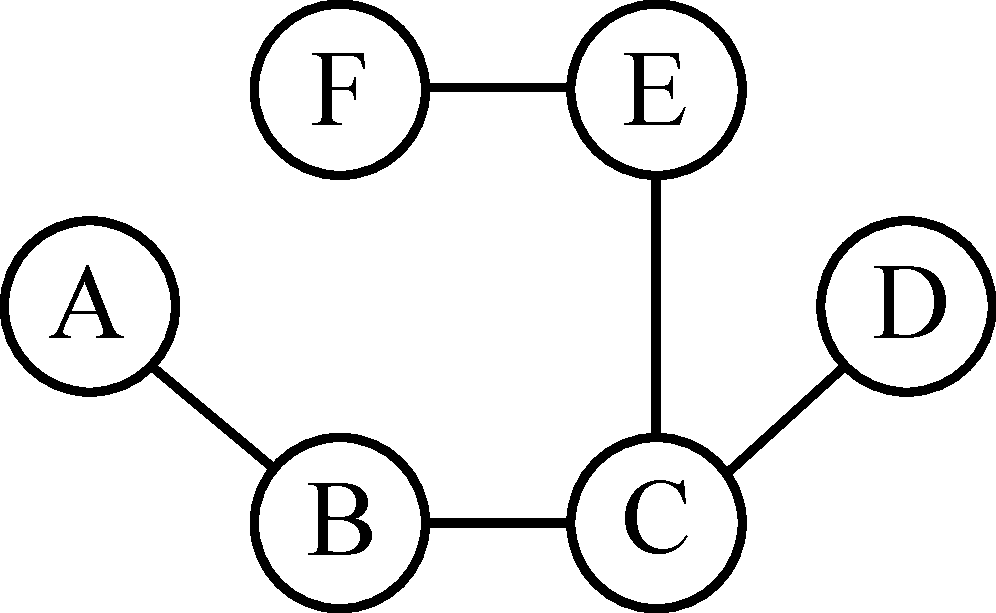
\includegraphics[width = .4\textwidth]{graph2.pdf}
\caption{An example of an minimum spanning tree for the previous graph}
\label{mst:graph2}
\end{figure}

\begin{figure}[H]
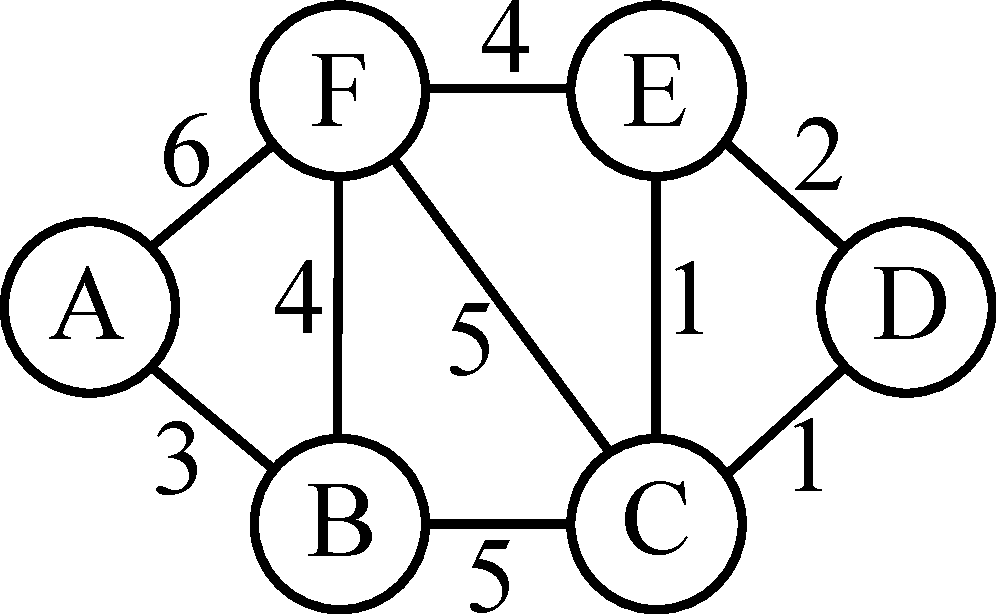
\includegraphics[width = .4\textwidth]{graph4.pdf}
\caption{A weighted directed graph}
\label{mst:graph4}
\end{figure}

\begin{figure}[H]
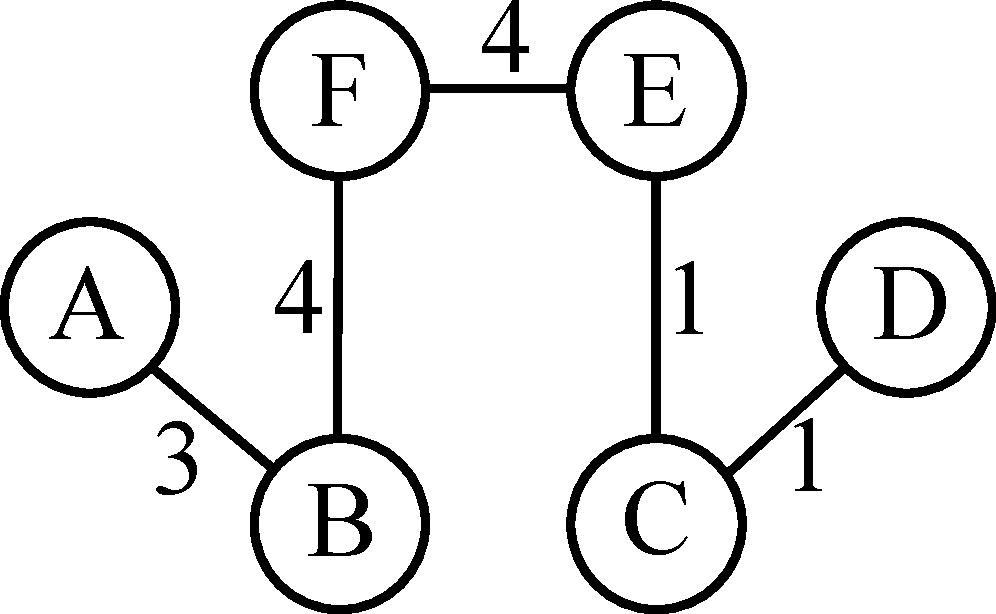
\includegraphics[width = .4\textwidth]{graph5.pdf}
\caption{The MST of the graph in Figure \ref{mst:graph4}.}
\end{figure}

\section*{Kruskal's algorithm}

Given a weighted directed graph G with $n$ nodes, Kruskal's algorithm finds the minimum by: first sorting the edges from smallest to largest.
Then, starting from the smallest, the algorithm adds the edge to the tree as long as the addition of the new edge does not create a cycle.
When $n-1$ edges have been added, the algorithm stops.

In order to avoid creating cycles while building the tree, it is necessary to keep track of which portions of the tree currently lie in connected groups.
This can be done by creating a dictionary, where, at the beginning, each node points to itself ans the "root" of its own tree.
As you add  edges into the tree you will change the "root" nodes of the nodes to show which nodes are currently connected.
Doing it in this way lets you run the algorithm by iterating over the edges by weight in ascending order, adding them to the tree if they connect nodes that are not already connected by the current tree.
As you build the tree, you could iterate over the nodes each time you add in a new edge.
That should be avoided.
It  is better to just change the "root" values of the previous roots as you go.

Consider the graph in Figure \ref{mst:graph4}.
Applying Kruskal's algorithm, the first step to finding a minimum spanning tree is to sort the edges by weight.
The result is something like the list \li{[(C,D,1),(C,E,1),(D,E,2),(A,B,3),(B,F,4),(E,F,4),(B,C,5),(C,F,5),(A,F,6)]}.
We initialize our tree to be an empty list \li{[]}.
To track the root nodes of each tree, we will also initialize a dictionary where each node points to itself.
It will look like this: \li{\{A:A,B:B,C:C,D:D,E:E,F:F\}}.
Since there are 6 nodes in the graph, we will continue until we have 5 edges in the tree.

Now we begin iterating through the edges to build the tree.
The first edge in the list is \li{(C,D,1)}.
The root for \li{C} is \li{C} and the root for \li{D} is \li{D}, so we add this edge into the tree, so the tree is \li{[(C,D,1)]}.
We then change the root node of \li{D} to be \li{C}.
The dictionary of root nodes now looks like \li{\{A:A,B:B,C:C,D:C,E:E,F:F\}}.

Now we process the next edge, \li{(C,E,1)}.
The root node of \li{C} is \li{C}, and the root node of \li{E} is \li{E}, so adding this edge does not create a cycle.
We add this edge into the tree, so the tree is now \li{[(C,D,1),(C,E,1)]}.
Then we change the root of \li{E} so that it is \li{C}, so the dictionary is \li{\{A:A,B:B,C:C,D:C,E:C,F:F\}}.

The next edge is \li{(D,E,2)}.
The root node of the tree containing \li{D} is \li{C} and the root node of the tree containing \li{E} is \li{C}, so these nodes are already connected, so we do not add this edge into the graph.

The next ege is \li{(A,B,3)}.
The root node for \li{A} is A, and the root node for \li{B} is \li{B}, so we add the edge in and update the dictionary.
The dictionary becomes \li{\{A:A,B:A,C:C,D:C,E:C,F:F\}}

The next edge is \li{(B,F,4)}.
The root node for \li{B} is \li{A} and the root node for \li{F} is \li{F}, so we add the edge in and change the root node of \li{F} to be \li{A}.
The dictionary becomes \li{\{A:A,B:A,C:C,D:C,E:C,F:A\}}

The next edge is \li{(E,F,4)}.
The root node for \li{E} is \li{C} and the root node for \li{F} is \li{A}.
We add in the edge and end the algorithm since there are now 5 edges.
If we were to continue the algorithm, we would update the root node of \li{A} to be \li{C}.

Notice how we just updated the root of the root node for one of the nodes in the edge we just added.
In order to find the root node of \li{F} we must trace back through the dictionary until we find a node that points to itself.
For example, the way we would now find the root node of \li{F} is to get the value for \li{F} from the dictionary, which is \li{A}, then get the value for \li{A} from the dictionary, which is \li{C}.
The value of \li{C} in the dictionary is itself, so it is the root node of the graph containing \li{F}.
It is necessary to trace through the dictionary in this manner each time to find the root nodes we need at each iteration because it lets us avoid iterating over all of the nodes and updating their root values each time.

Here is the pseudocode for the algorithm as we have described it above:

\begin{itemize}

\item Initialize an empty list of edges for the minimum spanning tree.

\item Make a dictionary that points each node toward its root (not always directly to it).
Start with each node pointing to itself.

\item Initialize the number of nodes that still need to be processed to the number of nodes minus 1.

\item Define a helper function that traces through the dictionary to find the root of its tree.
This can be done like this:

	\begin{itemize}

	\item Initialize a temporary variable to be the node for which we are finding the root.

	\item While the temporary node does not point to itself in the dictionary:

		\begin{itemize}

		\item Update the temporary node to be the node it currently points to in the dictionary.

		\end{itemize}

	\item return the temporary node

	\end{itemize}

\item Iterate over the edges by ascending weight (Use a \li{for} loop for this and just return the tree when it is big enough. That will break the loop for you.)

	\begin{itemize}

	\item Trace through the dictionary to find the root node of each of the nodes in the edge you are processing.

	\item If the roots are not the same:

		\begin{itemize}

		\item Add the edge to the tree

		\item Lower the number of edges remaining by one

		\item If the number of edges remaining is 0, return the tree (which also breaks the loop).

		\item Update the root of the root of the second node in the edge to be the root of the first node in the edge.

		\end{itemize}

	\end{itemize}

\end{itemize}
Note on implementation: You can iterate over a sorted copy of a list using the built in \li{sorted} function.
You can sort by the third value in each tuple using the \li{itemgetter} function that is part of the \li{operator} library included with Python.
For example:
\begin{lstlisting}
from operator import itemgetter
...
for n1, n2, weight in sorted(edges, key=itemgetter(2)):
    ...
\end{lstlisting}

\begin{problem}
Write Kruskal's algorithm.
Test your algorithm on random symmetric matrices.
Use the graph above and the data from MSTdata.npy to test your tree.
Use np.load("MSTdata.npy") to get it.
Use the formChanger function to put it in the right form.
% describe what formChanger does
\end{problem}

\section*{Prim's algorithm}

Prim's algorithm accomplishes the same thing as Kruskal's algorithm, but it uses a different approach.
Starting from any node it adds the edge with the least weight.
Those two nodes form a tree.
It than adds edges with the least weight to any node in the tree to any node not in the tree until all the nodes have been added.
The fastest way to do this is as follows:

\begin{itemize}

% Revise algorithm description

\item Start with the smallest-weight edge $e = \{x, y\}$ in $S$

\begin{itemize}

\item discard $x$ and $y$ from the list of nodes to consider

\item for both $x$ and $y$, find the closest node, if any (among the non-discarded nodes), and keep them and their edge weights

\end{itemize}

\item Until $n-1$ edges have been added

\begin{itemize}

\item Find the edge $e = \{x, y\}$ such that:

\begin{itemize}

\item $x$ is in $S$ and $y$ is not in $S$

\item $e$ is the smallest weighted edge left

\end{itemize}

\item add $e$ and $y$ to $S$

\item discard y from the list of nodes to consider, and for both $x$ and $y$, find the closest node, if any (among the non-discarded nodes), and keep them and their edge weights

\end{itemize}

\end{itemize}

\begin{problem}
Write Prim's algorithm.
Test your implementation with the same data as the previous problem.
Compare the speed of Prim's algorithm with Kruskal's algorithm. 
\end{problem}

\section*{Complexity}

Let $n$ be the number of nodes and $m$ be the number of edges.
Kruskal's Algorithm is O($m\log{n}$) which in the worst case is O($n^2\log{n}$).
Prims's Algorithm is O($n^2$).
So when the adjacent matrix is sparse Kruskal's is better and when it is dense Prim's is better. 